\subsection{The Classification Task}
We start by presenting the results of the classification task.
The classification task, unlike the detection task, assumes that an approximate location of an amino acid is given. 
Though the detection task is the more interesting one, analysis of the simpler classification task is key  to understanding the algorithm behavior and improving its performance.

Once trained, the CNN is used to perform prediction on a validation dataset, which is disjoint from the training set.
For each input cube with known label $j$, the softmax CNN produces "probabilities" $p_k$, $k=0,\cdots,C$.
The predicted label $i$ the one giving maximal "probability", and the confidence is $p_i$.

\subsubsection{Confusion Matrix and Reliability Curve}
For an amino acid labeled $j$, we are interested in the following questions:
\begin{enumerate}
\item  What are our chances to detect it correctly, and what are the chances of missing it with an amino acid $i$?
\item Does our confidence level $p_j$ reflect the probability of the true detection? Namely, does a $p_j$ fraction of all the inputs predicted as $j$ represent correct predictions.
\end {enumerate}
Commonly accepted tools for quantitative answers to these questions are the \textbf{confusion matrix} \cite{Fawcett2006AnAnalysis} and the \textbf{reliability  curve} \cite{Guo2017OnNetworks}.

An entry $a_{i,j}$  of a \textbf{confusion matrix} $A$ is defined as the ratio  $a_{i,j} = \frac{T_j^j}{N_j}$,  where  $N_j$ is the number of input cubes labeled $j$ and  $T_j^i$ the number of inputs labeled $j$ with predicted label $i$.
An ideal classification algorithm will result in $a_{i,i}=1$ and $a_{i,j}=0$ if $i\neq j$.
We also refer to $a_{i,i}$ as the \textbf{total accuracy} of label $i$.

It is desired that softmax CNN be \textbf{well calibrated} \cite{Guo2017OnNetworks}, i.e., the predicted confidence should reflect the ground truth probability.
A \textbf{reliability curve} is a plot of ground truth accuracy prediction vs reported confidence. 
For a perfectly calibrated network the probability curve is an identity function. 
For the experimental results the ground truth accuracy is estimated by grouping predictions in interval bins according to their reported confidence \cite{Guo2017OnNetworks}. 
\subsubsection{$2.2 \AA$ Resolution}

\paragraph{Simulation Results}
We start by analyzing the results  obtained on simulated data.
Though it is commonly accepted that simulated data is not as reliable as real data, analysis of classification CNN performance on simulated data provides important insight on the real data behavior.
Also, simulated data results provide an upper limit of what can be achieved with the selected CNN architecture.

Figure ~\ref{f:CM_22_SS} shows the confusion matrix obtained while the total accuracies are summarized in Figure ~\ref{f:ss22_acc}.
The amino acids with the highest accuracy are: LEU, GLY, ALA, VAL, LYS, TYR, PRO.
This indicates that the number of rotamers \cite{Shapovalov2011ARegressions} of an amino acid has a major effect on the accuracy.
Since an amino acid with a large number of rotamers can exhibit numerous conformations, it is harder for a classification algorithm to adjust its parameters for the given amino acid.
Except LYS, all of the above amino acids have a relatively small number of rotamers. 
Moreover, all the amino acids with a small number of rotamers have high classification accuracy,  except Glutamic acid and Glutamine which are mutually mixed in classification.
The size of the dataset is another dominant factor for the classification accuracy. 
In a Machine Learning approach a large training dataset enables robust parameter estimation and reduces the effect of overfitting.
Figures ~\ref{f:DS_22_SS} and ~\ref{f:DS_norm_22_SS} show the correlation between the training dataset size and the resulting accuracy.

\begin{figure}[!ht]
\begin{minipage}[b]{0.45\linewidth}
\begin{subfigure}[b]{\linewidth}
	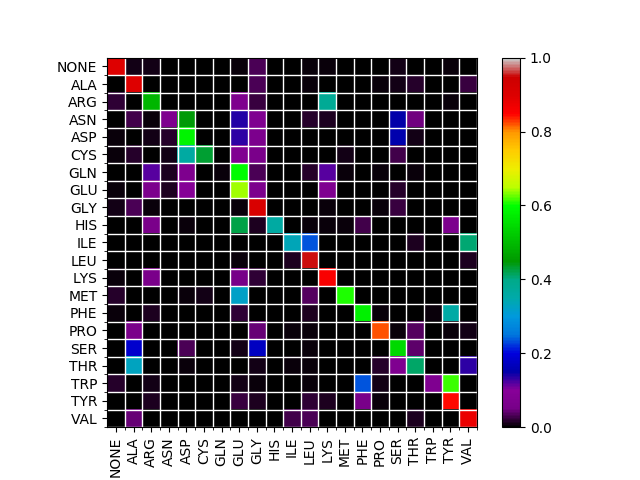
\includegraphics[width=1.27\textwidth]{pics/CM_22_SS}
	\caption{Confusion Matrix}
	\label{f:CM_22_SS}
\end{subfigure}
\end{minipage}
\begin{minipage}[b]{0.45\linewidth}
\begin{subfigure}[b]{\linewidth}
	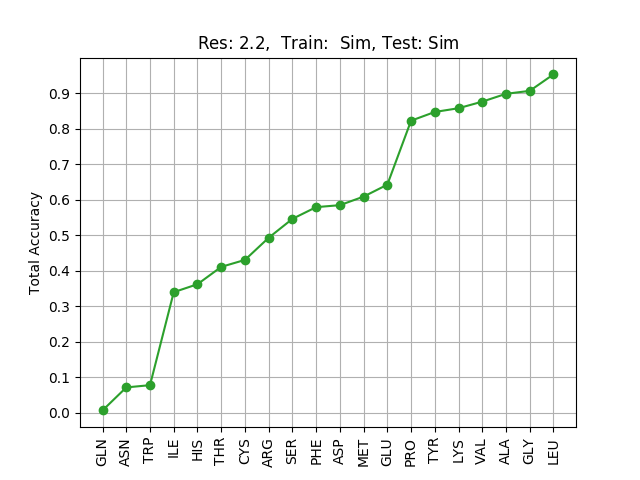
\includegraphics[width=1.27\textwidth]{pics/ss22_acc.png}
	\caption{Total Accuracy}
	\label{f:ss22_acc}
\end{subfigure}
\end{minipage}
\caption{Classification Results: Resolution $2.2 \AA$,  Train: Simulated, Test : Simulated}
\end{figure}

\begin{figure}[!ht]
\begin{minipage}[b]{0.45\linewidth}
\begin{subfigure}[b]{\linewidth}
	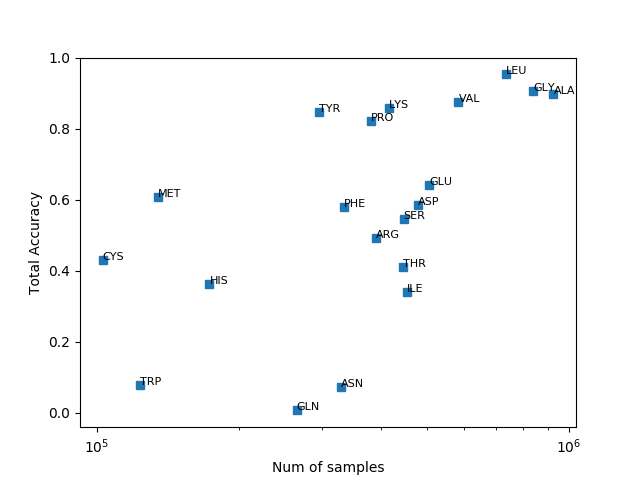
\includegraphics[width=1.1\textwidth]{pics/DS_22_SS}
	\caption{Accuracy vs Dataset size \newline \newline}
	\label{f:DS_22_SS}
\end{subfigure}
\end{minipage}
\begin{minipage}[b]{0.45\linewidth}
\begin{subfigure}[b]{\linewidth}
	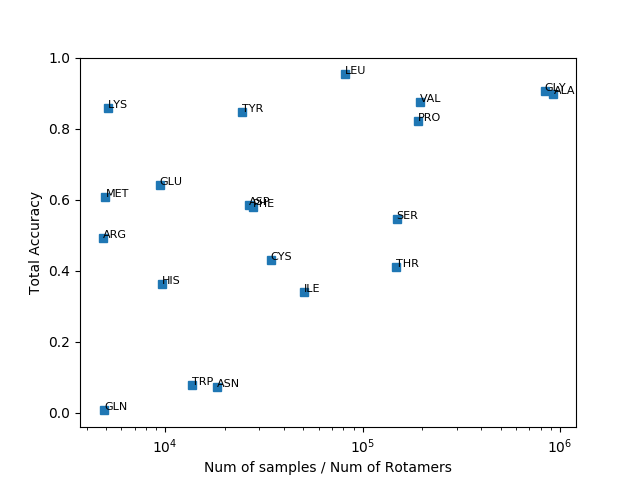
\includegraphics[width=1.1\textwidth]{pics/DS_norm_22_SS.png}
	\caption{Accuracy vs Dataset size normalized to the number of Rotamers}
	\label{f:DS_norm_22_SS}
\end{subfigure}
\end{minipage}
\caption{Effect of the Training Dataset Size on the Classification Accuracy: Resolution $2.2 \AA$,  Train: Simulated, Test : Simulated}
\end{figure}


\paragraph{Experimental Data Results}
We used a $2.2$ cryo-EM map of $\beta$-galactosidase (\cite{Bartesaghi20152.2Inhibitor}. EMD-2984) to study the CNN performance.
At the time of the research, only three additional cryoEM maps with resolution better than $2.3 \AA$ were available: EMD-8762 \cite{Dong2017Antibody-inducedB14},EMD-8194 \cite{Merk2016BreakingDiscovery}, and EMD-3295 \cite{Banerjee20162.3Inhibition}.
Even augmented , this is definitely not enough for proper training of the CNN.
The confusion matrix and the total accuracies are shown in Figures ~\ref{f:CM_22_RR} and ~\ref{f:rr22_acc}.
The accuracy dependence on the dataset size is shown in Figures ~\ref{f:DS_22_RR} and ~\ref{f:DS_norm_22_RR}.
Despite significantly lower accuracies, the tendency observed on simulated data is preserved.

In order to improve the classification accuracy we tried two methods to overcome the lack of data:
\begin{enumerate}
\item We trained up to 6 independent CNNs and averaged the obtained probabilities.
\item We combined the real maps with the simulated maps and created  a new dataset.
\end{enumerate}
The first method, averaging over multiple networks, did not result in any significant improvement of the classification accuracy.
This indicates that the obtained low accuracy is not due to overfitting, but due to the small training set.
Best classification results were achieved by combining in the training set simulated and experimental data in equal proportion.
We denote the CNN trained on this combined dataset as $N^{22}_{ES}$.
The detection accuracies for this case are shown in Figures ~\ref{f:CM_22_RSR} and ~\ref{f:rsr22_acc}.

Figure ~\ref{f:rl_22} shows the estimated reliability curves for $N^{22}_{ES}$. 
Due to lack of data, reliability curves cannot be estimated for every input, but the overall tendency is that the output of the softmax layer of $N^{22}_{ES}$ underestimated the classification accuracy.

\begin{figure}[!ht]
\begin{minipage}[b]{0.45\linewidth}
\begin{subfigure}[b]{\linewidth}
	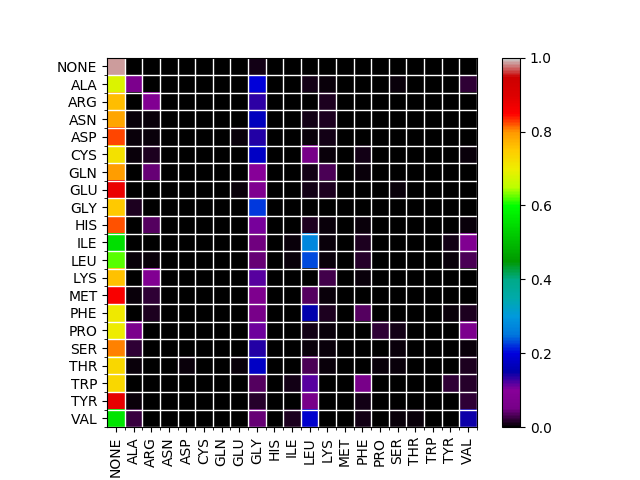
\includegraphics[width=1.27\textwidth]{pics/CM_22_RR}
	\caption{Confusion Matrix}
	\label{f:CM_22_RR}
\end{subfigure}
\end{minipage}
\begin{minipage}[b]{0.45\linewidth}
\begin{subfigure}[b]{\linewidth}
	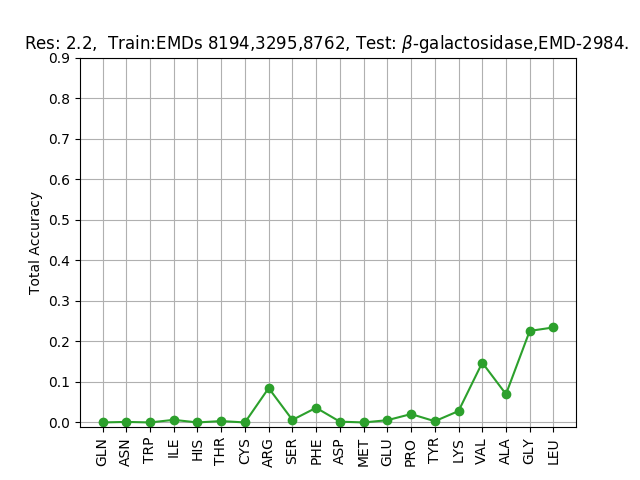
\includegraphics[width=1.27\textwidth]{pics/rr22_acc.png}
	\caption{Total Accuracy}
	\label{f:rr22_acc}
\end{subfigure}
\end{minipage}
\caption{Classification Results: Resolution $2.2 \AA$,  Train: EMDs 8762,3295,8184, Test : $\beta$-galactosidase, \cite{Bartesaghi20152.2Inhibitor}. }
\end{figure}

\begin{figure}[!ht]
\begin{minipage}[b]{0.45\linewidth}
\begin{subfigure}[b]{\linewidth}
	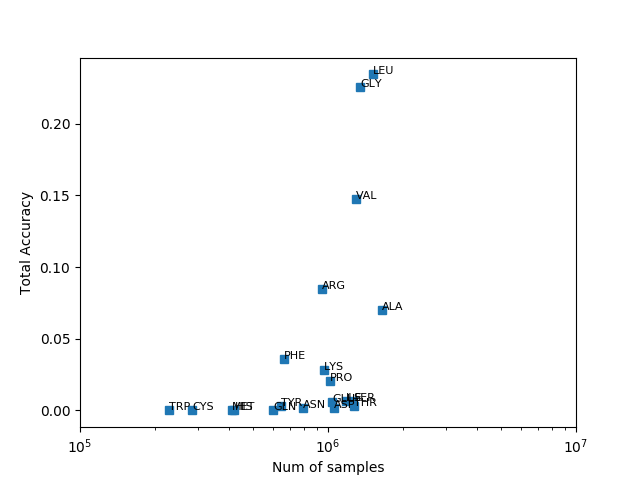
\includegraphics[width=1.1\textwidth]{pics/DS_22_RR}
	\caption{Accuracy vs Dataset size \newline \newline}
	\label{f:DS_22_RR}
\end{subfigure}
\end{minipage}
\begin{minipage}[b]{0.45\linewidth}
\begin{subfigure}[b]{\linewidth}
	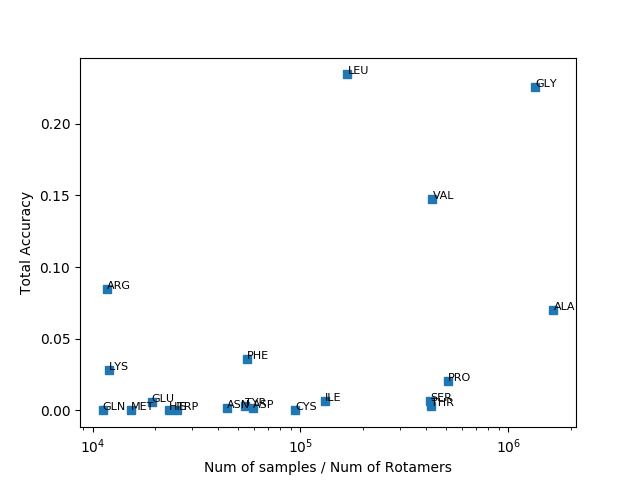
\includegraphics[width=1.1\textwidth]{pics/DS_norm_22_RR.png}
	\caption{Accuracy vs Dataset size normalized to a number of Rotamers}
	\label{f:DS_norm_22_RR}
\end{subfigure}
\end{minipage}
\caption{Effect of Training Dataset Size on the Classification Accuracy: Train: EMDs 8762,3295,8184, Test : $\beta$-galactosidase, \cite{Bartesaghi20152.2Inhibitor}.}
\end{figure}


\begin{figure}[!ht]
\begin{minipage}[b]{0.45\linewidth}
\begin{subfigure}[b]{\linewidth}
	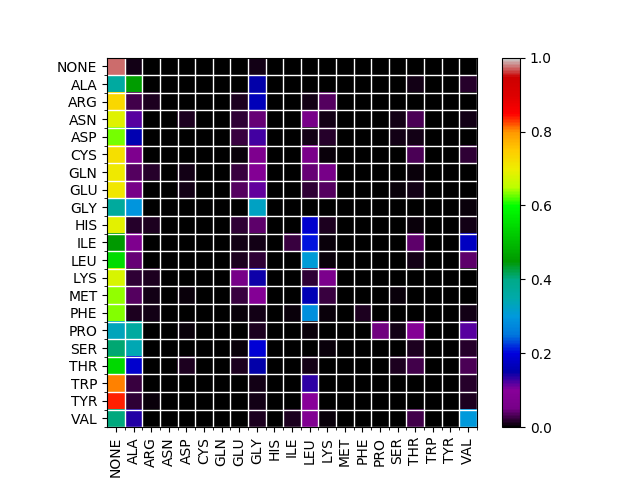
\includegraphics[width=1.27\textwidth]{pics/CM_22_RSR}
	\caption{Confusion Matrix}
	\label{f:CM_22_RSR}
\end{subfigure}
\end{minipage}
\begin{minipage}[b]{0.45\linewidth}
\begin{subfigure}[b]{\linewidth}
	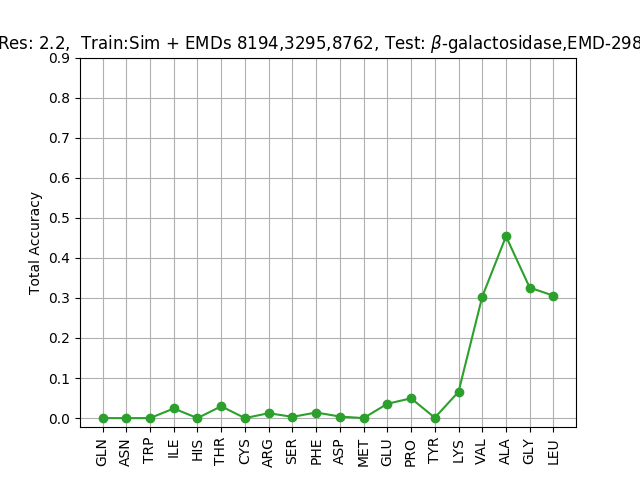
\includegraphics[width=1.27\textwidth]{pics/rsr22_acc.png}
	\caption{Total Accuracy}
	\label{f:rsr22_acc}
\end{subfigure}
\end{minipage}
\caption{Classification Results: Resolution $2.2 \AA$,  Train: Simulation + EMDs 8762,3295,8184, Test : $\beta$-galactosidase, \cite{Bartesaghi20152.2Inhibitor}. }
\end{figure}

\begin{figure}[!ht]
\begin{minipage}[b]{0.45\linewidth}
\begin{subfigure}[b]{\linewidth}
	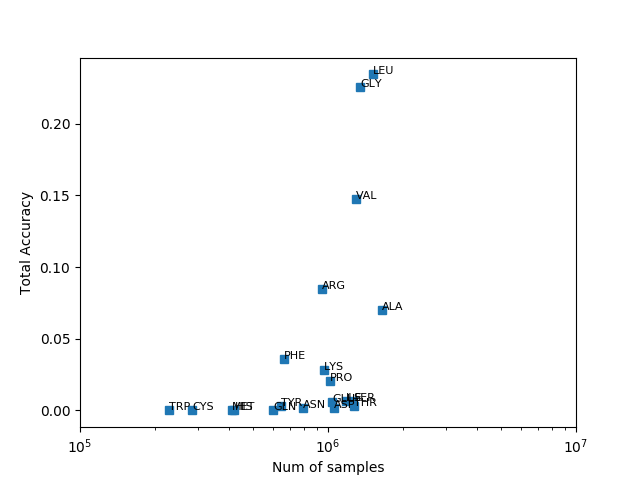
\includegraphics[width=1.1\textwidth]{pics/DS_22_RR}
	\caption{Accuracy vs Dataset size \newline \newline}
	\label{f:DS_22_RR}
\end{subfigure}
\end{minipage}
\begin{minipage}[b]{0.45\linewidth}
\begin{subfigure}[b]{\linewidth}
	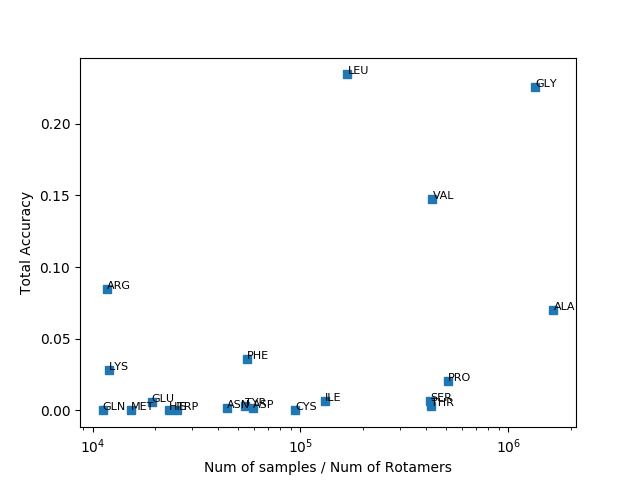
\includegraphics[width=1.1\textwidth]{pics/DS_norm_22_RR.png}
	\caption{Accuracy vs Dataset size normalized to the number of Rotamers}
	\label{f:DS_norm_22_RR}
\end{subfigure}
\end{minipage}
\caption{Effect of Training Dataset Size on the Classification Accuracy: Train: EMDs 8762,3295,8184, Test : $\beta$-galactosidase, \cite{Bartesaghi20152.2Inhibitor}.}
\end{figure}


\begin{figure}[!ht]
\begin{minipage}[b]{0.45\linewidth}
\begin{subfigure}[b]{\linewidth}
	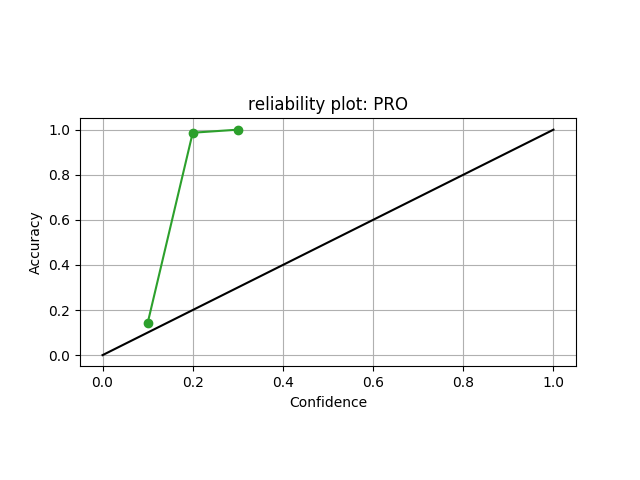
\includegraphics[width=1.27\textwidth]{pics/rel_PRO_22_SRS}
\end{subfigure}
\begin{subfigure}[b]{\linewidth}
	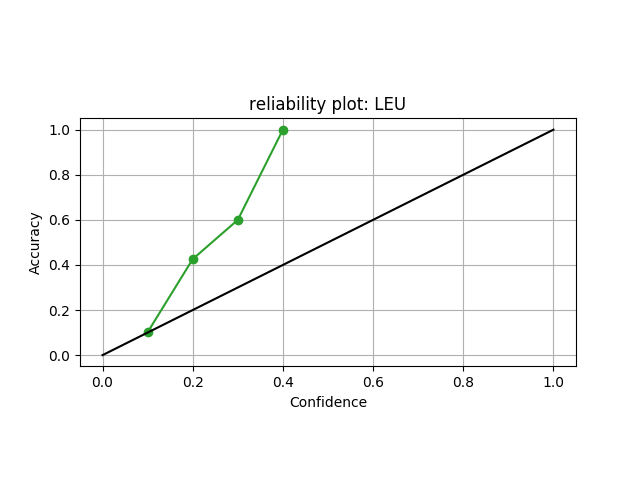
\includegraphics[width=1.27\textwidth]{pics/rel_LEU_22_SRS}
\end{subfigure}

\end{minipage}
\begin{minipage}[b]{0.45\linewidth}
\begin{subfigure}[b]{\linewidth}
	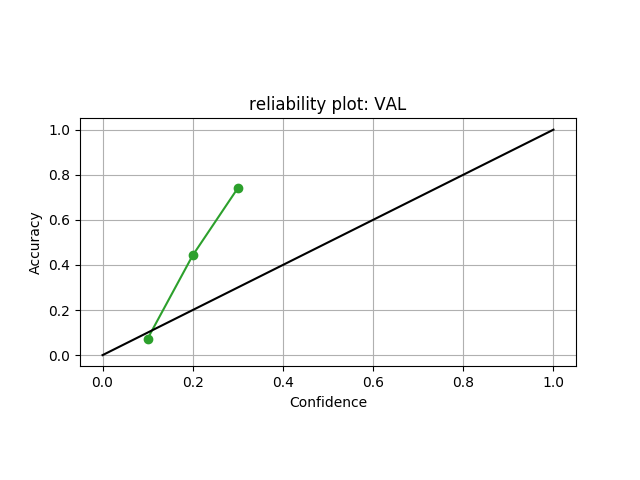
\includegraphics[width=1.27\textwidth]{pics/rel_VAL_22_SRS}
\end{subfigure}
\begin{subfigure}[b]{\linewidth}
	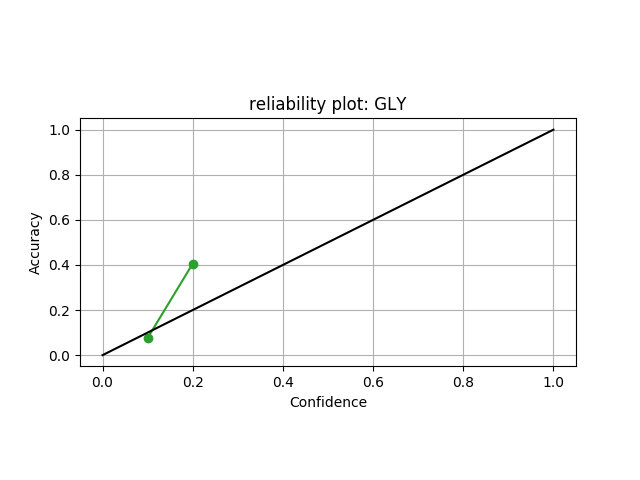
\includegraphics[width=1.27\textwidth]{pics/rel_GLY_22_SRS}
\end{subfigure}
\end{minipage}
\caption{Estimated Reliability Curves for PRO, LEU, VAL, GLY : Resolution $2.2 \AA$,  Train: Simulation + EMDs 8762,3295,8184, Test : $\beta$-galactosidase, \cite{Bartesaghi20152.2Inhibitor}. }\label{f:rl_22}
\end{figure}


\subsubsection{Resolutions $2.9 \AA$ and   $3.1 \AA$ }
Coarsening the resolution has two opposite effects on the classification accuracy.
Intuitively, in higher resolution maps the amino acids shape is sharper, but lower resolution maps benefit from a larger training dataset.
The size of the training dataset for three tested resolutions is shown on Table ~\ref{t0}.
The effect of a map resolution on the classification accuracy is shown in Figures ~\ref{f:s3_293_acc} and ~\ref{f:r3_293_acc}.
While having only a small effect on simulated data (Figure ~\ref{f:s3_293_acc}), the effect of resolution on the real data is well expressed (Figure ~\ref{f:r3_293_acc}).
 Accuracies for $2.9 \AA$ and $3.1 \AA$ are significantly better than those for $2.2 \AA$. This is clearly due to the increased training dataset. 
 The only exception is Alanin, which is probably too small to be detected at resolutions above $2.2 \AA$.
However, moving from $2.9 \AA$ to $3.1 \AA$ we see that for the majority of the amino acids the total accuracy values are decreased.  Thus, in this transition the effect of increasing the training dataset size did not compensate for the degradation in map precision.
 
The confusion matrices for $2.9 \AA$ Anthrax toxin protective antigen pore and $3.1 \AA $ Lysenin Pore are presented in Figures ~\ref{f:CM_29_RR} and ~\ref{f:CM_31_RR}, respectively. The Reliability Curves for the $2.9 \AA$ Anthrax toxin protective antigen pore and $3.1 \AA $ Lysenin Pore are presented in Figures ~\ref{f:CM_29_RR} ~\ref{f:CM_31_RR}, respectively.
 While at resolution of $2.9 \AA$ the estimated confidence is still less than the observed one, at $3.1 \AA$ resolution the estimated confidence is of good precision.
 
\begin{table}
\begin{tabular}{ | m{5em} | m{3cm} | m{3cm}| }
\hline
 Resolution Span & Maps in Training Set  & Map for Validation \\
\hline
 $1.8-2.3 \AA$  & 3  & EMD-2984 , $2.2 \AA$ $beta$ -galactosidase \cite{Banerjee20162.3Inhibition} \\
\hline
 $2.7-2.9 \AA$  & 8  & EMD-6224 ,$2.9 \AA$  Anthrax toxin protective antigen pore \cite{jiang2015atomic} \\
\hline
 $2.9-3.1 \AA$  & 13  & EMD -8015, $3.1 \AA$ Lysenin Pore \cite{Bokori-Brown2016Cryo-EMProtein} \\
\hline
 \end{tabular}
\caption{Experimental Train and Test data for Various Resolutions}\label{t0}
\end{table}

\begin{figure}[!ht]
\begin{minipage}[b]{0.45\linewidth}
\begin{subfigure}[b]{\linewidth}
	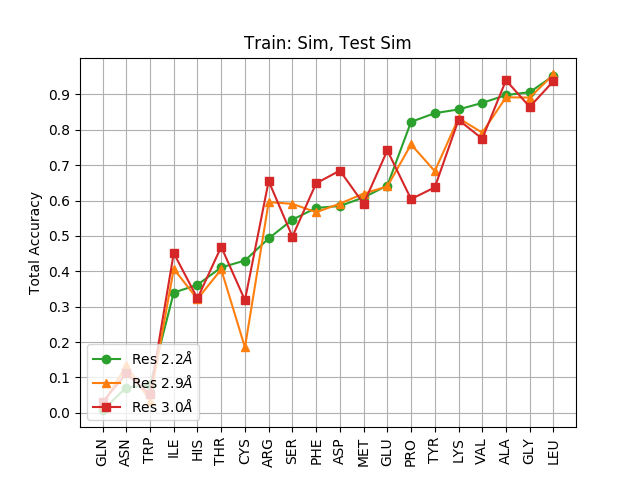
\includegraphics[width=1.1\textwidth]{pics/s3_293_acc}
	\caption{Simulated Data \newline \newline}
	\label{f:s3_293_acc}
\end{subfigure}
\end{minipage}
\begin{minipage}[b]{0.45\linewidth}
\begin{subfigure}[b]{\linewidth}
	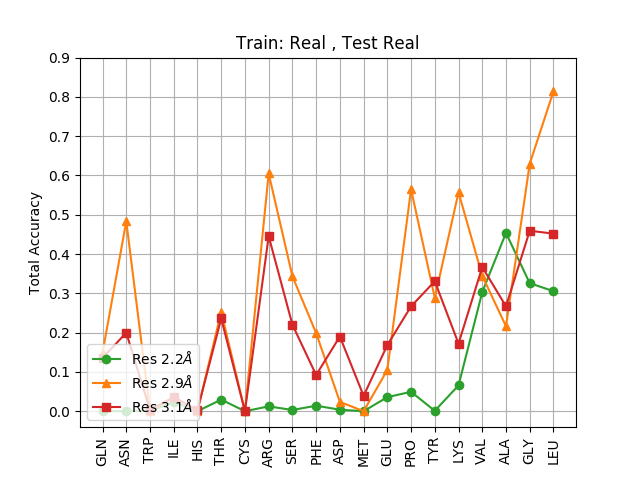
\includegraphics[width=1.1\textwidth]{pics/r3_293_acc}
	\caption{Real Data (Mixed with Simulation for Resolution $2.2 \AA$}
	\label{f:r3_293_acc}
\end{subfigure}
\end{minipage}
\caption{Total classification accuracies for different resolutions.}
\end{figure}


\begin{figure}[!ht]
\begin{minipage}[b]{0.45\linewidth}
\begin{subfigure}[b]{\linewidth}
	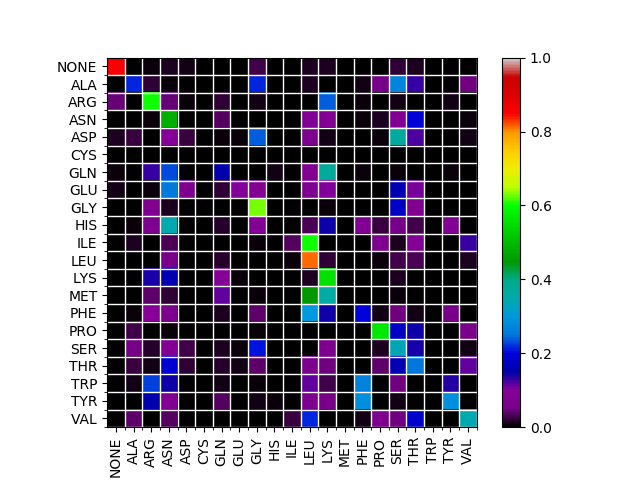
\includegraphics[width=1.2\textwidth]{pics/CM_29_RR}
	\caption{Accuracy vs Dataset size \newline \newline}
	\label{f:CM_29_RR}
\end{subfigure}
\end{minipage}
\begin{minipage}[b]{0.45\linewidth}
\begin{subfigure}[b]{\linewidth}
	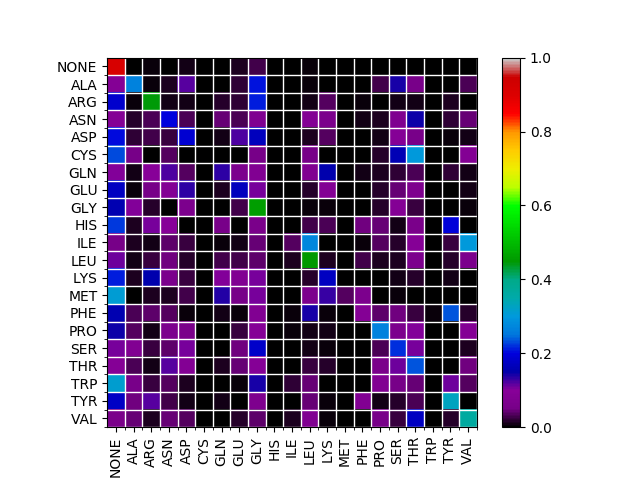
\includegraphics[width=1.2\textwidth]{pics/CM_31_RR.png}
	\caption{Accuracy vs Dataset size normalized to a number of Rotamers}
	\label{f:CM_31_RR}
\end{subfigure}
\end{minipage}
\caption{Classification Accuracy Results for Resolution $2.9$ and $3.1$ }
\end{figure}

\begin{figure}[!ht]
\begin{minipage}[b]{0.45\linewidth}
\begin{subfigure}[b]{\linewidth}
	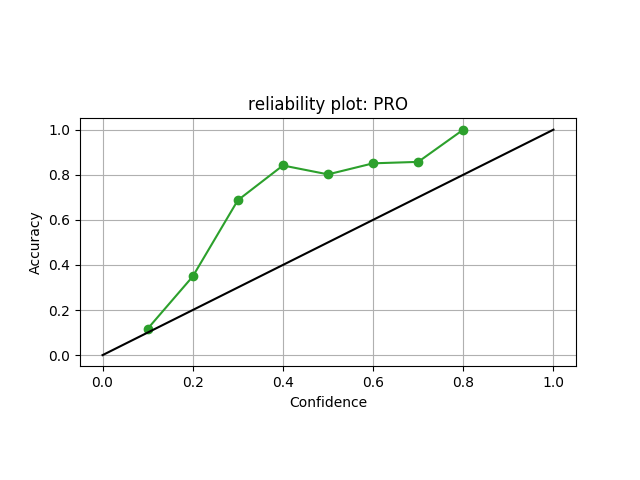
\includegraphics[width=1.27\textwidth]{pics/rel_PRO_29_RR}
\end{subfigure}
\begin{subfigure}[b]{\linewidth}
	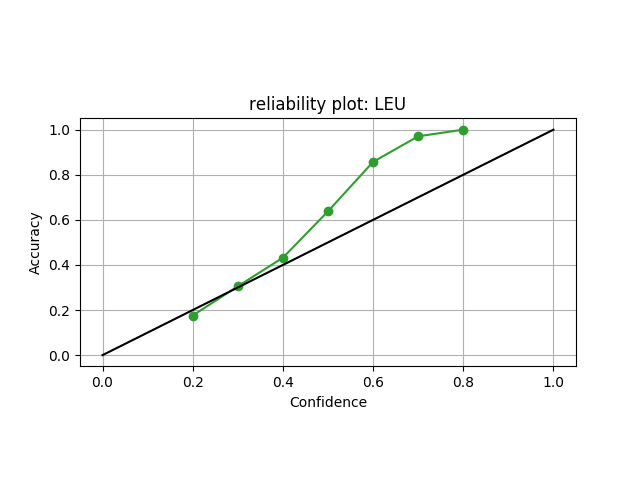
\includegraphics[width=1.27\textwidth]{pics/rel_LEU_29_RR}
\end{subfigure}

\end{minipage}
\begin{minipage}[b]{0.45\linewidth}
\begin{subfigure}[b]{\linewidth}
	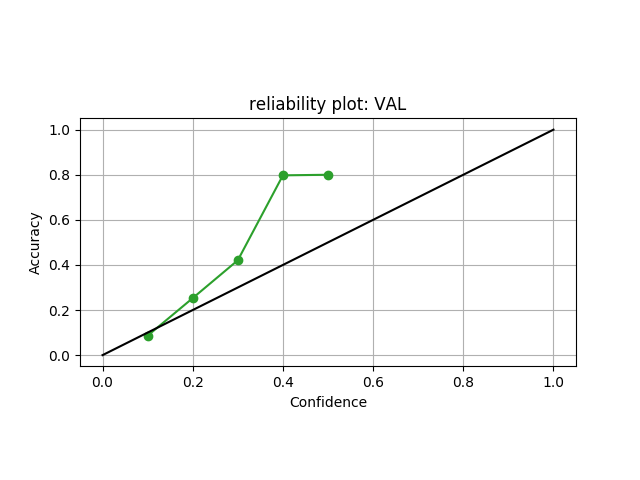
\includegraphics[width=1.27\textwidth]{pics/rel_VAL_29_RR}
\end{subfigure}
\begin{subfigure}[b]{\linewidth}
	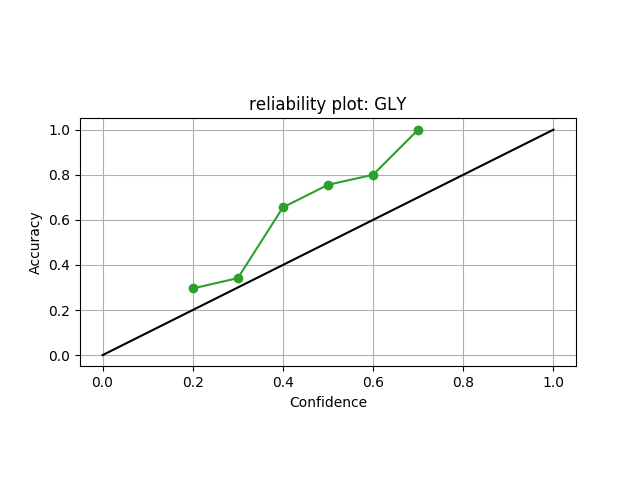
\includegraphics[width=1.27\textwidth]{pics/rel_GLY_29_RR}
\end{subfigure}
\end{minipage}
\caption{Estimated Reliability Curves for PRO, LEU, VAL, GLY : Resolution $2.9 \AA$,  Train: Experimental Data, Test :  Anthrax toxin protective antigen pore \cite{jiang2015atomic}.}\label{f:rl_29}
\end{figure}

\begin{figure}[!ht]
\begin{minipage}[b]{0.45\linewidth}
\begin{subfigure}[b]{\linewidth}
	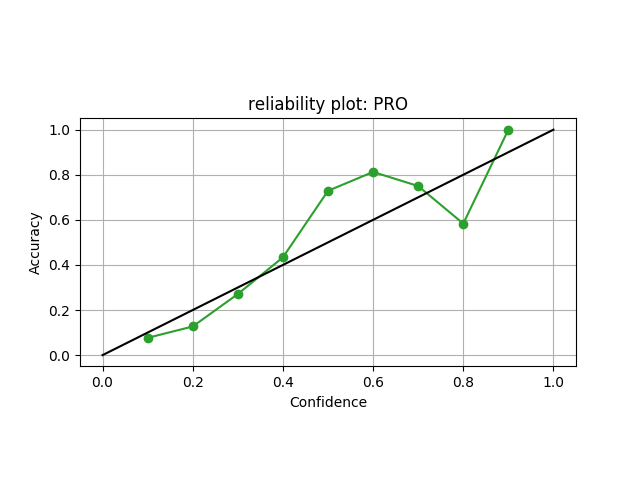
\includegraphics[width=1.27\textwidth]{pics/rel_PRO_31_RR}
\end{subfigure}
\begin{subfigure}[b]{\linewidth}
	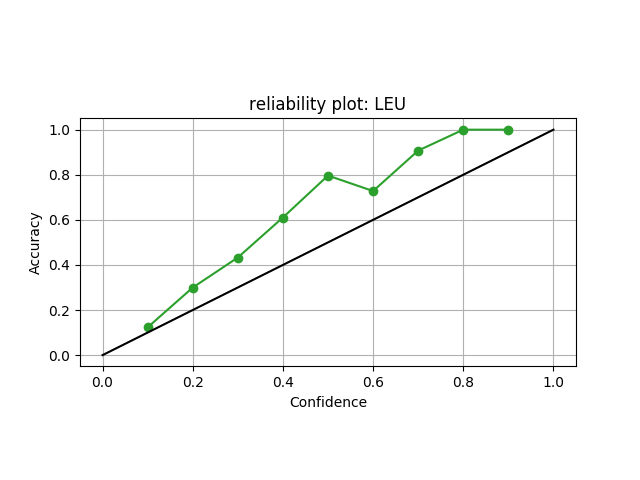
\includegraphics[width=1.27\textwidth]{pics/rel_LEU_31_RR}
\end{subfigure}

\end{minipage}
\begin{minipage}[b]{0.45\linewidth}
\begin{subfigure}[b]{\linewidth}
	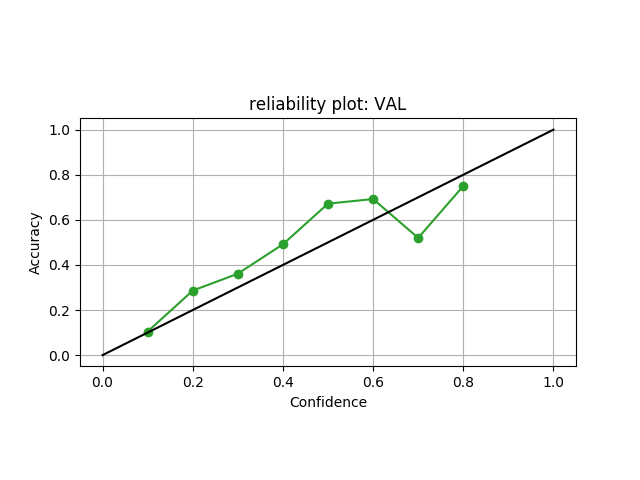
\includegraphics[width=1.27\textwidth]{pics/rel_VAL_31_RR}
\end{subfigure}
\begin{subfigure}[b]{\linewidth}
	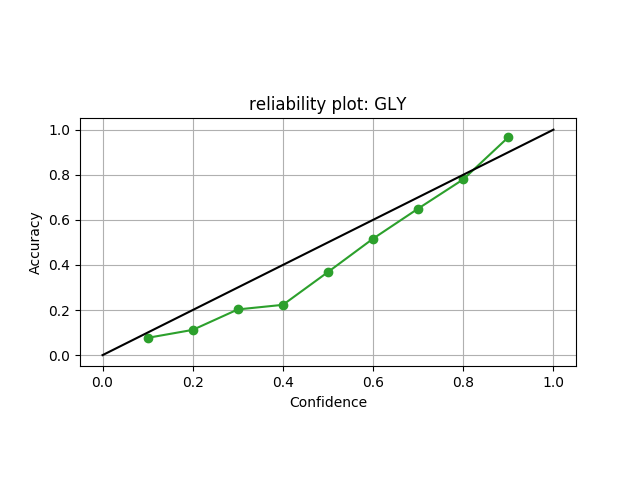
\includegraphics[width=1.27\textwidth]{pics/rel_GLY_31_RR}
\end{subfigure}
\end{minipage}
\caption{Estimated Reliability Curves for PRO, LEU, VAL, GLY : Resolution $3.1 \AA$,  Train: Experimental Data, Test :  Lysenin Pore \cite{Bokori-Brown2016Cryo-EMProtein}. }\label{f:rl_31}
\end{figure}


\subsection{Detection Results}
In the detection (also called localization) task, the exact location of an amino acid is unknown. 
Whilst the localization of all amino acids of a protein seems to be a hard problem at this time, detection of a subset of the amino acids obtained with high confidence is achievable. 
In this paper we focused on identifying \textbf{anchors}, i.e., amino acids, which have been located and labeled with confidence above $80 \%$. 


For each resolution case we tested a number of different classification methods, while the pre-processing and post-processing phases remain unchanged.

Table ~\ref{t22} summarizes the detection picks for the $2.2\AA$ map of $beta$-galactosidase \cite{Bartesaghi20152.2Inhibitor}.  
There we succeed to detect amino acids of four types: ARG, LEU, PRO, VAL with confidence above $80\%$.
The fraction of the detected high confidence amino acids is up to $10 \%$ from the total amount of the same type.
We expect this result to improve, as more high resolution cryo EM maps are being released.


Table \ref{t29} summarizes the detection picks for the test map of the $2.9\; \AA$ resolution anthrax toxin protective antigen pore \cite{jiang2015atomic}.  
We succeded to detect $70 \%$ of the Prolines.
Figure ~\ref{f:PRO29} illustrates the results of proline detection.
The detection rate of ARG, LEU, TYR,VAL was about $20 \%$.

Table \ref{t31} summarizes the detection picks for the test map of $3.1 \; \AA$ resolution Lysenin Pore \cite{Bokori-Brown2016Cryo-EMProtein}.
We detected more than $20 \%$ of the Leucine residues.
We also succeded to detect about $10 \%$ of LYS, TYR, ARG, GLY and PRO.
Figure ~\ref{f:LYS31} illustrates the detection results for LEU, LYS, TYR and GLY at map resolution of $3.1 \AA$.

Note that the use of simulated data was crucial for the $2.2 \AA$ resolution experiment.
For resolutions $2.9 \AA$ and   $3.1 \AA$ the role of simulated data is less important, since more experimental maps are available.

\begin{table}
\small
\begin{tabular}{ | m{4em} | m{1.5cm} || m{1.5cm}|| m{2.6cm}| } 
 \hline
 Amino Acid Type & Picks with Confidence of $80\%$   & Total in Protein & Best Method \\
 \hline
\hline
ARG  & 17  & 133 & $maj(N_S,N_E,N_{ES})$  \\
\hline
LEU  & 15    & 231 & $mean(N_S,N_E,N_{ES})$   \\
\hline
PRO  & 10    & 189 & $N_{ES}$  \\
\hline
VAL  & 10    & 119 & $mean(N_S,N_E,N_{ES})$  \\
\hline
\end{tabular}
\caption{Detection Results $2.2 \; \AA$ cryo-EM single particle reconstruction of beta galactosidase (emd-2984)}\label{t22}
\end{table}


\begin{table}
\begin{tabular}{ | m{4em} | m{1.5cm} || m{1.5cm}|| m{2.6cm}| } 
 \hline
 Amino Acid Type & Picks with Confidence of $80\%$  & Total in Protein & Best Method \\
 \hline
\hline
ASN  & 5    & 287 & $N_E$  \\
\hline
ARG  & 20    & 119 & $N_E$  \\
\hline
LEU  & 40    & 231 & $N_E$  \\
\hline
LYS  & 30    & 189 & $mean(N_S,N_E)$  \\
\hline
PRO  & 80  & 133 & $maj(N_S,N_E,N_{ES})$  \\
\hline
TYR  & 18    & 91 & $N_{ES}$  \\
\hline
VAL  & 35    & 161 & $N_E$  \\
\hline
\end{tabular}
\caption{Detection results for $2.9 \; \AA$ CryoEM single particle reconstruction of an "anthrax toxin protective antigen pore (emd-6224)"}\label{t29}
\end{table}

\begin{table}
\begin{tabular}{ | m{4em} | m{1.5cm} || m{1.5cm}|| m{2.6cm}| } 
 \hline
 Amino Acid Type & Picks with Confidence of $80\%$  & Total in Protein & Best Method \\
 \hline
\hline
ARG  & 10  & 117 & $N_{ES}$  \\
\hline
GLY  & 25  & 207 & $N_E$  \\
\hline
LEU  & 25  & 108 & $N_E$  \\
\hline
LYS  & 20  & 171 & $N_E$  \\
\hline
PRO  & 9  & 72 & $mean(N_R,N_E)$  \\
\hline
TYR  & 18  & 144 & $maj(N_R,N_E,N_{ES})$  \\
\hline

\end{tabular}
\caption{Detection results for $3.1 \; \AA$ CryoEM single particle reconstruction of an "Lysenin Pore (emd-8015)"}\label{t31}
\end{table}

\begin{figure}
  \caption{Proline detection in  $2.9 \; \AA$ CryoEM single particle reconstruction of an "anthrax toxin protective antigen pore (emd-6224). Purple regions indicate the detected proline residues} \label{f:PRO29}
  \centering
    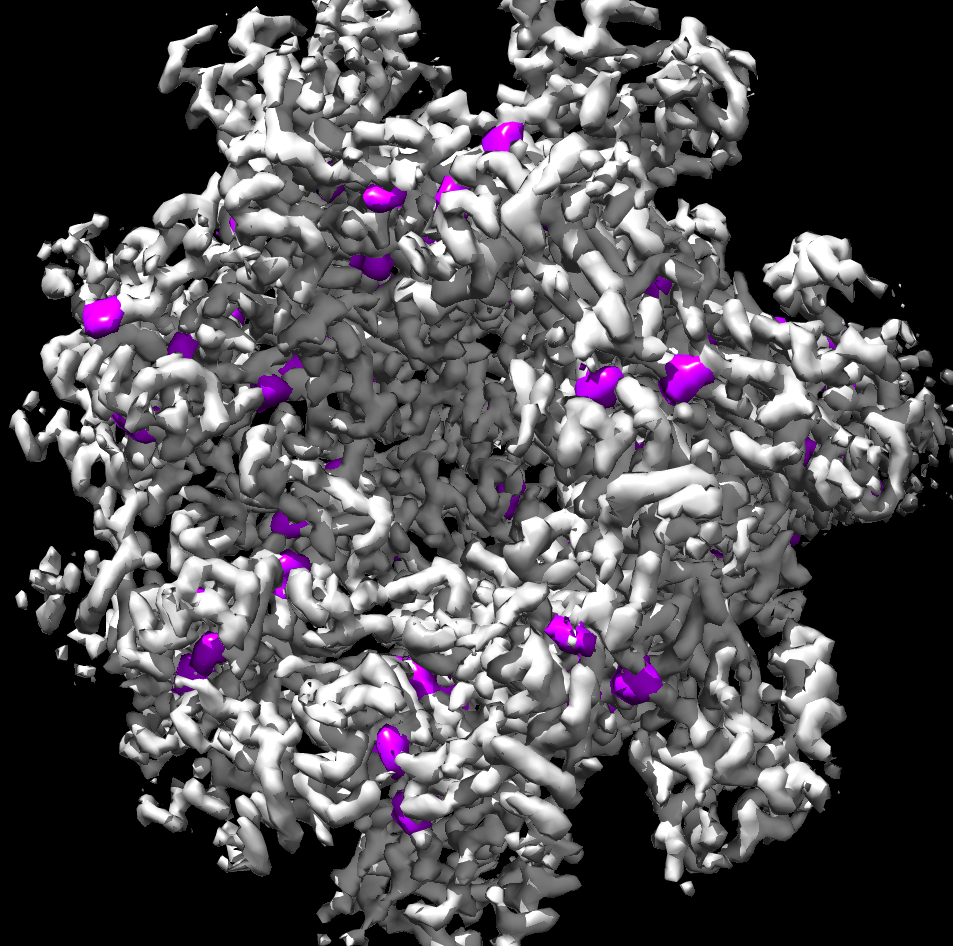
\includegraphics[width=0.5\textwidth]{pics/map_PRO.png}
\end{figure}

\begin{figure}
  \caption{Detection leucines, lysines, glycines and tyrosines  in  $3.1 \; \AA$ CryoEM single particle reconstruction of single particle reconstruction of an "Lysenin Pore (emd-8015)". Red regions indicate the detected {\color{red} leucines}, blue regions indicate the detected {\color{blue} lysines}, yellow regions indicate the detected {\color{yellow} glycines}, and green regions indicate the detected {\color{green} tyrosines} } \label{f:LYS31}
  \centering
    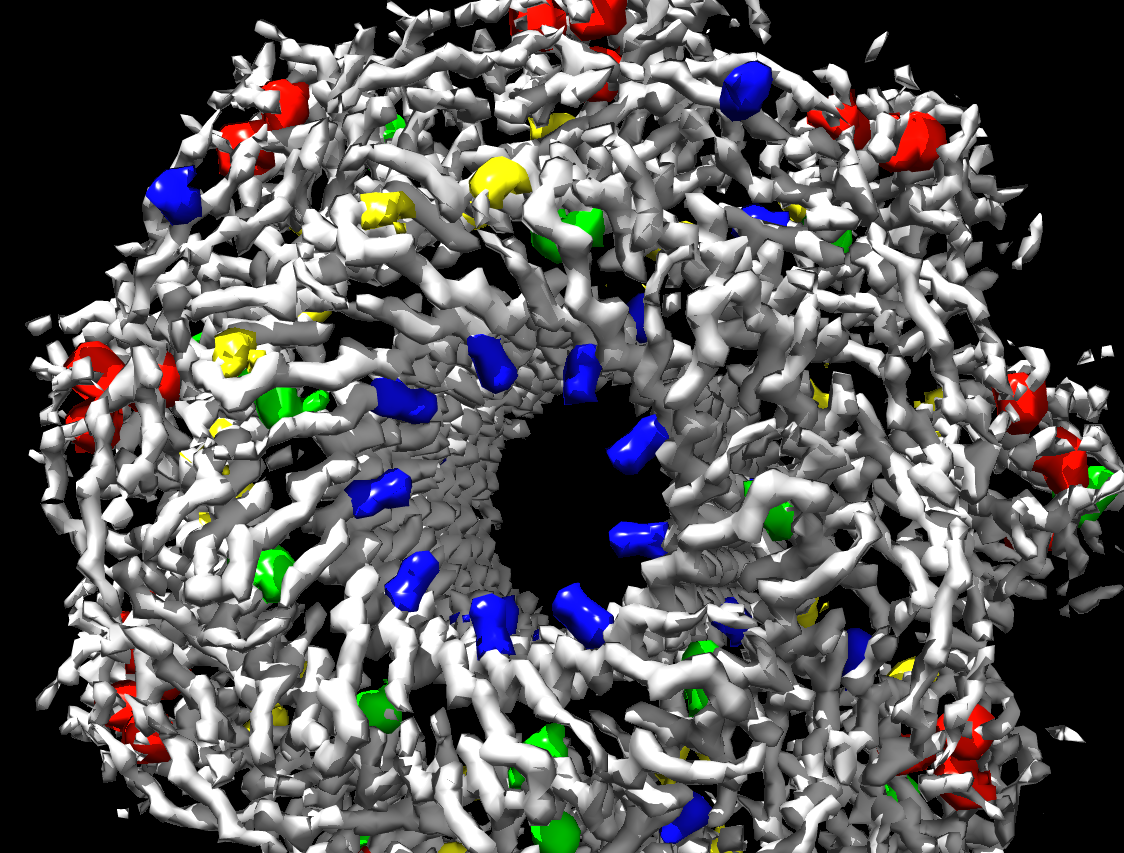
\includegraphics[width=0.5\textwidth]{pics/lys_pore_GLY_LEU_LYS_TYR.png}
\end{figure}

% Denote by 
% For our analysis we use the following quantities:
% \begin{itemize}
% 	\item \textbf{Recall} or hit rate (also true positive rate) for a label $j$ defined as $R(j) = \frac{T_j^j}{N_j}$
%     \item text
% \end{itemize}



% \subsection{Detection}
% \subsubsection{Resolution 2.2 Detection Results}
% \subsection{Precision- Recall curves}
% Precision (P) is defined as the number of true positives ($T_p$) over the number of true positives plus the number of false positives ($F_p$).
% $$
% P = \frac{T_p}{T_p+F_p}
% $$

% Recall ($R$) is defined as the number of true positives ($T_p$) over the number of true positives plus the number of false negatives ($F_n$).

% $$ R = \frac{T_p}{T_p + F_n} $$